\documentclass[pdftex,12pt,a4paper]{article}
\usepackage[pdftex]{graphicx}
\usepackage{xcolor}
\usepackage{marginnote}
\usepackage{enumitem}
\usepackage{multirow}
\usepackage{subcaption}
\usepackage{titlesec}
\usepackage[bottom=1.5cm, outer=5cm, inner=2cm, heightrounded,
marginparwidth=4cm, marginparsep=0.5cm]{geometry}
\titleformat{\section}{\bfseries}{\Large Question \thesection: }{0em}{}

\begin{document}
    % Custom title page
    \begin{titlepage}
        \begin{center}
            
\includegraphics[width=5cm]{figures/kulogo}\\[1cm]
            {\large \bfseries
                Spring 2014\\
                Computer Networks\\
                CMPE323\\[1cm]
            }
            {\large \bfseries
                \noindent Quiz 2\\[1cm]
            }
        \end{center}

        \begin{center}
            \begin{tabular}{|c|p{1cm}l|}\hline
                \textbf{Questions} & \multicolumn{2}{|c|}{\textbf{Points}} \\\hline
                Q1                &    &    /80\%   \\\hline
                Q2                &    &    /20\%   \\\hline
            \end{tabular}
        \end{center}

        \vfill
        \begin{tabular}{lp{5cm}ll}
            \textbf{Student name:} & & \textbf{Student ID:} & \\
        \end{tabular}


    \end{titlepage}
    \newpage

    % quiz content
    \section{}
        Consider Figure \ref{fig1} where the network is correctly configured
        to allow PC1 and PC2 to communicate.

        \begin{figure}[tbh]
            \centering
            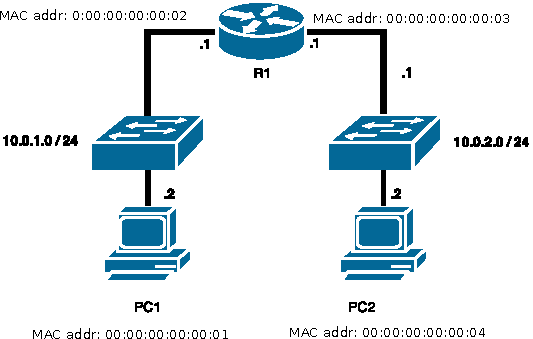
\includegraphics[width=.85\textwidth]{figures/diag1}
            \caption{Two PCs in two broadcast domains that are interconnected
            by a single router.}
            \label{fig1}
        \end{figure}

        Additionally, suppose that PC1 initiated some TCP connection against
        PC2's port 80. The dynamically chosen source port number by PC1 was
        40,000. The TCP three-way hand-shake has progressed so far as depicted
        in Figure \ref{fig:tcpsyn}.

        \begin{figure}[tbh]
        \centering
        \small\begin{verbatim}   PC 1                                                 PC 2 
1. CLOSED                                               LISTEN
2. SYN-SENT    --> <SEQ=1><CTL=SYN>                 --> SYN-RECEIVED
3. ESTABLISHED <-- <SEQ=300><ACK=2><CTL=SYN,ACK>    <-- SYN-RECEIVED
4. ESTABLISHED -->                ???               --> ESTABLISHED\end{verbatim}\normalsize
       \vspace{-15pt}
       \caption{TCP's three-way hand-shake for connection establishment between
       PC1 and PC2.}
       \label{fig:tcpsyn}
       \end{figure}

       \textbf{The question is:} what data should PC1 send to PC2 in order to complete
       the TCP three-way hand-shake (i.e. step 4 from Figure \ref{fig:tcpsyn}). Answer this question by filling the
       Figures \ref{fig:eth}, \ref{fig:ipv4} and \ref{fig:tcp} in the next page as follows:
       \begin{itemize}
           \item Only fill fields that are marked by an
               asterisk ``\texttt{*}'', and ignore the others.
           \item The protocol type for IP is \texttt{0x0800}.
           \item The protocol type for TCP is \texttt{0x06}.
       \end{itemize}

       \textbf{Grading scheme:} every field that is correctly filled rewards
       you with 5 points. I.e. correctly filling all of the 16 fields will
       give you $5 \times 16 = 80$ points.

        \begin{figure}[!h]
        \centering
        \small\begin{verbatim} 0                   1                   2                   3
 0 1 2 3 4 5 6 7 8 9 0 1 2 3 4 5 6 7 8 9 0 1 2 3 4 5 6 7 8 9 0 1
+-+-+-+-+-+-+-+-+-+-+-+-+-+-+-+-+-+-+-+-+-+-+-+-+-+-+-+-+-+-+-+-+
|  *Source MAC address                                          |
+                               +-+-+-+-+-+-+-+-+-+-+-+-+-+-+-+-+
|                               |  *Destination MAC address     |
+-+-+-+-+-+-+-+-+-+-+-+-+-+-+-+-+                               +
|                                                               |
+-+-+-+-+-+-+-+-+-+-+-+-+-+-+-+-+-+-+-+-+-+-+-+-+-+-+-+-+-+-+-+-+
|  *Type                        |                               
+-+-+-+-+-+-+-+-+-+-+-+-+-+-+-+-+\end{verbatim}\normalsize
        \vspace{-15pt}
        \caption{Ethernet frame (only fill the value of fields that are marked
        with an asterisk ``\texttt{*}'').}
        \label{fig:eth}
        \end{figure}

        \begin{figure}[!h]
        \centering
        \small\begin{verbatim} 0                   1                   2                   3
 0 1 2 3 4 5 6 7 8 9 0 1 2 3 4 5 6 7 8 9 0 1 2 3 4 5 6 7 8 9 0 1
+-+-+-+-+-+-+-+-+-+-+-+-+-+-+-+-+-+-+-+-+-+-+-+-+-+-+-+-+-+-+-+-+
|Version|  IHL  |Type of Service|          Total Length         |
+-+-+-+-+-+-+-+-+-+-+-+-+-+-+-+-+-+-+-+-+-+-+-+-+-+-+-+-+-+-+-+-+
|         Identification        |Flags|      Fragment Offset    |
+-+-+-+-+-+-+-+-+-+-+-+-+-+-+-+-+-+-+-+-+-+-+-+-+-+-+-+-+-+-+-+-+
|  Time to Live | *Protocol     |         Header Checksum       |
+-+-+-+-+-+-+-+-+-+-+-+-+-+-+-+-+-+-+-+-+-+-+-+-+-+-+-+-+-+-+-+-+
|                      *Source Address                          |
+-+-+-+-+-+-+-+-+-+-+-+-+-+-+-+-+-+-+-+-+-+-+-+-+-+-+-+-+-+-+-+-+
|                   *Destination Address                        |
+-+-+-+-+-+-+-+-+-+-+-+-+-+-+-+-+-+-+-+-+-+-+-+-+-+-+-+-+-+-+-+-+\end{verbatim}\normalsize
        \vspace{-15pt}
        \caption{IPv4 header (only fill the value of fields that are marked
        with an asterisk ``\texttt{*}'').}
        \label{fig:ipv4}
        \end{figure}

        \begin{figure}[!h]
        \centering
        \small\begin{verbatim} 0                   1                   2                   3
 0 1 2 3 4 5 6 7 8 9 0 1 2 3 4 5 6 7 8 9 0 1 2 3 4 5 6 7 8 9 0 1
+-+-+-+-+-+-+-+-+-+-+-+-+-+-+-+-+-+-+-+-+-+-+-+-+-+-+-+-+-+-+-+-+
|         *Source Port          |      *Destination Port        |
+-+-+-+-+-+-+-+-+-+-+-+-+-+-+-+-+-+-+-+-+-+-+-+-+-+-+-+-+-+-+-+-+
|                       *Sequence Number                        |
+-+-+-+-+-+-+-+-+-+-+-+-+-+-+-+-+-+-+-+-+-+-+-+-+-+-+-+-+-+-+-+-+
|                   *Acknowledgment Number                      |
+-+-+-+-+-+-+-+-+-+-+-+-+-+-+-+-+-+-+-+-+-+-+-+-+-+-+-+-+-+-+-+-+
|       |           |*|*|*|*|*|*|                               |
|  Data |           |U|A|P|R|S|F|                               |
| Offset| Reserved  |R|C|S|S|Y|I|            Window             |
|       |           |G|K|H|T|N|N|                               |
|       |           | | | | | | |                               |
+-+-+-+-+-+-+-+-+-+-+-+-+-+-+-+-+-+-+-+-+-+-+-+-+-+-+-+-+-+-+-+-+
|           Checksum            |         Urgent Pointer        |
+-+-+-+-+-+-+-+-+-+-+-+-+-+-+-+-+-+-+-+-+-+-+-+-+-+-+-+-+-+-+-+-+\end{verbatim}\normalsize
        \vspace{-15pt}
        \caption{TCP header (only fill the value of fields that are marked
        with an asterisk ``\texttt{*}'').}
        \label{fig:tcp}
        \end{figure}

        \pagebreak

    \section{}
        Following the scenario in Figures \ref{fig1} and \ref{fig:tcpsyn}, and
        in the context of TCP communication, how would PC2 behave if it did not
        receive an \texttt{ACK} message from PC1 for a relatively long time
        period?



\end{document}
